\documentclass[11pt]{article}
\usepackage[T1]{fontenc}
\usepackage{lmodern}
\usepackage[margin=0.95in]{geometry}
\usepackage{amsmath,amssymb}
\usepackage{microtype}
\usepackage{enumitem}
\usepackage{needspace}
\usepackage{xcolor}
\usepackage[most]{tcolorbox}
\usepackage{tikz}
\usetikzlibrary{positioning,arrows.meta,decorations.pathreplacing}
\usepackage[colorlinks=true,linkcolor=blue!50!black]{hyperref}

\newcommand{\C}{\mathbb{C}}
\newcommand{\R}{\mathbb{R}}
\newcommand{\inner}[2]{\langle #1,#2\rangle}
\newcommand{\abs}[1]{\lvert #1\rvert}
\newcommand{\norm}[1]{\lVert #1\rVert}
\newcommand{\Frob}{\mathrm{F}}
\DeclareMathOperator{\U}{U}
\newcommand{\key}[1]{\par\Needspace{4\baselineskip}\medskip\noindent{\normalsize\bfseries #1}\par\nobreak\vspace{-1pt}}

\title{\bfseries From a point of $\U(2)$ to two more bases\\[5pt]
\large\normalfont How the covering of Step 2 decides whether a third and fourth basis exist\\[3pt]
\normalsize\itshape Companion to \texttt{mub-outline.pdf}, Steps 3--5; preprint \S6--7.
Only school mathematics is assumed}
\author{}
\date{}

\begin{document}
\maketitle

\noindent
Step 2 ends with a point of $\U(2)$ for every completion of a seed, and Step 3 covers $\U(2)$ by finitely
many cells. Neither says anything about a third or a fourth basis. This note explains how covering a
group of $2\times2$ matrices decides a question about two extra bases of $\C^6$ --- and what happens to
the matrices that a covering step refuses.

\smallskip
\noindent
\textbf{The short answer.} The covering turns ``all $6\times6$ Hadamard matrices'' into finitely many
\emph{boxes}, each a small neighbourhood of one explicit matrix. Inside a box every entry of $H$ is
pinned down to a known error, so the question ``does this $H$ extend by two further bases?'' becomes a
question about finitely many small balls of candidate vectors --- and that question is settled by a
finite graph test with one-sided power: it can prove that no two extra bases exist, never that they do.
A box that the test cannot refute is not thrown away; it is refined and tested again. The proof is
complete when no box is left unresolved.

\key{1.\ What would have to exist}

Fix the first two bases: the standard basis $e_1,\dots,e_6$, and the columns $h_1,\dots,h_6$ of
$H/\sqrt6$, where $H$ is a $6\times6$ matrix whose entries all have modulus $1$ and whose columns are
orthogonal of length $\sqrt6$ ($H^*H=6I_6$). Two bases are \emph{unbiased} when every overlap between
a vector of one and a vector of the other has modulus $1/\sqrt6$; the modulus-one entries of $H$ are
exactly what makes the second basis unbiased to the first. A third basis is a list $w_1,\dots,w_6$ of
unit vectors with
\[
\inner{w_i}{w_j}=0\ \ (i\ne j),\qquad
\abs{\inner{e_k}{w_j}}^2=\abs{\inner{h_k}{w_j}}^2=\tfrac16\ \ \text{for all }k,j .
\]
A fourth basis is six more vectors $w'_1,\dots,w'_6$, orthogonal among themselves, unbiased to the first
two bases, and unbiased to the third: $\abs{\inner{w_i}{w'_j}}^2=\tfrac16$ for all $36$ pairs. So the
question is whether twelve vectors exist with this pattern:
\begin{center}
\emph{six and six, orthogonal within each group, and all $36$ pairs across the groups unbiased.}
\end{center}
The condition $\abs{\inner{e_k}{w_j}}^2=1/6$ already forces every entry of every $w_j$ to have modulus
$1/\sqrt6$. That is what makes the candidates coverable in \S4.

\key{2.\ What Step 2 gives, and what it does not}

Step 2 attaches a point of $\U(2)$ to every completion, with no exception: inside a seed ball every
exact $H$ produces a point $V$ of $\U(2)$ --- the rigid-motion part of the unknown block --- and $V$ lies
within a computed distance $p<0.067$ of a point computed from the centre (the derivation is in
\texttt{mub-step2.pdf}, \S\S3--4). Here $\U(2)$ is the set of $2\times2$ complex matrices $V$ with
$V^*V=I_2$: the linear maps of $\C^2$ that preserve lengths and angles. None of the notation of Step 2
is needed here; only the output is.

\smallskip
\noindent
\textbf{Nothing is left uncovered.} The map from completions to $\U(2)$ has no gaps: every exact $H$
in an accepted seed ball produces a point. What can
fail is a \emph{computation} --- a frame check, or the size of the defect --- and a failed computation
produces an \emph{unresolved} seed, never an uncovered matrix. An unresolved seed is recorded, and the
run fails; the conclusion is drawn only from a run in which no seed is unresolved. The same rule
governs everything below: a test may discard a region only when \emph{no} exact object in it can pass.

\smallskip
\noindent
\textbf{What Step 2 does not do} is decide anything about a third basis. It only says that once the seed
is fixed, the sixteen remaining phases cost four parameters rather than sixteen. That reduction is what
makes the boxes of the next section small enough to test.

\key{3.\ From a point of $\U(2)$ to a box of matrices}

Fix one seed ball and one cell of $\U(2)$. It is convenient to measure phases in \emph{cycles}, so that
a phase is a number modulo $1$; the seed ball then has radius $r_s=0.032$ cycles, which is
$R_s=2\pi r_s=0.201$ radians. Every exact $H$ belonging to this pair has its nine seed phases within
$r_s$ of the centre's, and its unknown block within $p<0.067$ of $\sqrt6$ times \emph{a point of the
cell}. Both statements are about entries, so they place all $36$ phases of $H$ in one ball of known
radius around an explicit matrix $P$ built from the centre and the cell, the cell's own width being one
of the terms in that radius.

That ball need not yet be small enough to test. The refinement passes of Stage B replace it by finitely
many smaller ones, \emph{certified phase balls}: a centre $P\in\R^{6\times6}$ (the $36$ phases), a
radius $r\le0.03$ cycles (that is $0.19$ radians), and a certificate that every exact $H$ in the ball
satisfies the orthogonality equations to within a stated defect. Those are the boxes.

Finitely many boxes cover everything, up to the four equivalences of Step 1 --- permuting rows or
columns, rephasing them, conjugating every entry, transposing --- and each of those preserves
extendibility, so refuting every box refutes every $H$. The whole chain is worth having in one picture.

\begin{center}
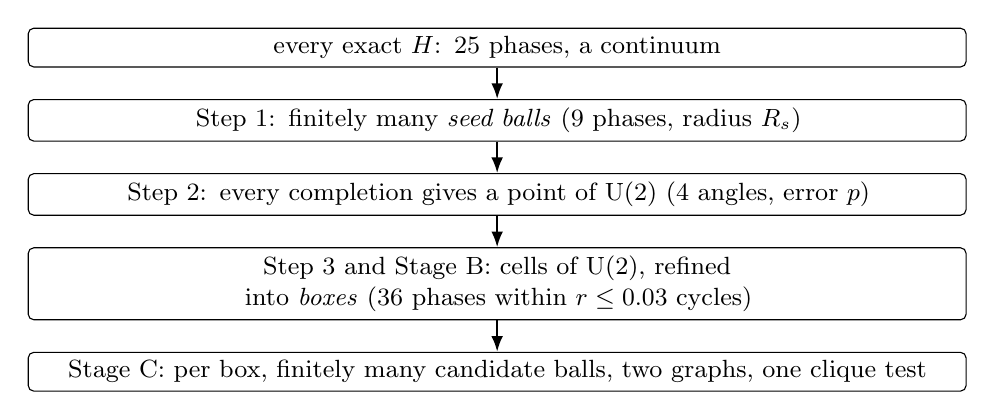
\begin{tikzpicture}[font=\small,
  box/.style={draw,rounded corners=2pt,text width=11.7cm,align=center,inner sep=3pt},
  ar/.style={-{Latex[length=2mm]},thick}]
\node[box] (a) {every exact $H$: $25$ phases, a continuum};
\node[box,below=4mm of a] (b) {Step 1: finitely many \emph{seed balls} ($9$ phases, radius $R_s$)};
\node[box,below=4mm of b] (c) {Step 2: every completion gives a point of $\U(2)$ ($4$ angles, error $p$)};
\node[box,below=4mm of c] (d) {Step 3 and Stage B: cells of $\U(2)$, refined into \emph{boxes} ($36$ phases within \mbox{$r\le0.03$} cycles)};
\node[box,below=4mm of d] (e) {Stage C: per box, finitely many candidate balls, two graphs, one clique test};
\foreach \x/\y in {a/b,b/c,c/d,d/e} \draw[ar] (\x)--(\y);
\end{tikzpicture}
\end{center}

\key{4.\ The candidates are finitely many balls}

A vector unbiased to the first basis has the form
\[
w=\frac1{\sqrt6}\bigl(e(x_1),\dots,e(x_6)\bigr),\qquad e(t)=e^{2\pi it},
\]
with $x_j$ the phase of the $j$-th entry. Multiplying $w$ by a unit complex number changes no overlap,
so we may fix $x_1=0$; five phases remain, each on a circle.

Cut each of the five circles into $M$ closed intervals. That gives $M^5$ closed boxes in the five
phases, hence $M^5$ closed balls of vectors, and every candidate vector lies in one of them. The
recorded run has four layers, $M=12\to24\to48\to96$, each finer than the last; at the first layer there
are $12^5\approx250{,}000$ boxes. The bins retained at the last layer are clustered into at most $2048$
balls, and those are the vertices below. The clustering is certified, not guessed: each retained bin is
assigned a ball whose radius provably covers it (the preprint's Lemma 6.4), and exceeding $2048$ balls,
or producing one of radius $0.1$ or more, is \emph{unresolved} --- never a discard.

Two vectors in one ball cannot be confused: if the radius is below $0.1$, their unnormalised inner
product has modulus more than $2.9$, whereas orthogonality needs $0$ and unbiasedness needs $\sqrt6$.
(The bound is the estimate of \S5, applied with both vectors in the same ball.) So the twelve vectors
of \S1, if they exist, occupy twelve \emph{different} balls --- which is why the pattern below is drawn
on distinct vertices. A single-vector test also discards a ball when no vector in it can be unbiased to
the second basis for any $H$ in the box.

\key{5.\ Two graphs, and the pattern}

Make one vertex for each ball that survives the single-vector test. Join two vertices by an
\emph{$O$-edge} when some vector in one ball and some vector in the other could be orthogonal; join them
by a \emph{$U$-edge} when the two could be unbiased. ``Could'' is decided by a test that errs in one
direction only: an edge is omitted just when an inequality proves that \emph{no} pair of vectors, one
from each ball, has the relation. Here is the test, and it is school algebra.

Let the two ball centres have phases $u_1,\dots,u_6$ and $v_1,\dots,v_6$, and let their radii be
$s_u,s_v$. For actual vectors in the balls, write their phases as $u_j+\xi_j$ and $v_j+\eta_j$ with
$\norm{\xi}\le s_u$ and $\norm{\eta}\le s_v$ (a ball's radius is measured in this Euclidean sense), and
put
\[
S=\sum_{j=1}^6 e(u_j-v_j),\qquad S'=\sum_{j=1}^6 e(u_j+\xi_j-v_j-\eta_j).
\]
The unnormalised inner product of the two vectors is $S'/6$, and $\abs{S'-S}\le2\pi\sqrt6\,(s_u+s_v)$,
by $\abs{e(t)-1}\le2\pi\abs t$, the triangle inequality and Cauchy--Schwarz. Orthogonality means
$S'=0$, so it forces
\[
\abs S\le2\pi\sqrt6\,(s_u+s_v)\qquad(O);
\]
unbiasedness means $\abs{S'}=\sqrt6$, so it forces
\[
\Bigl|\frac{\abs S}{\sqrt6}-1\Bigr|\le2\pi\,(s_u+s_v)\qquad(U).
\]
If the relevant inequality fails, that edge is impossible and is not drawn. With both vectors in the
same ball of radius $s$ the same bound gives $\abs{S'}\ge6-2\pi\sqrt6\,(2s)$, which exceeds $2.9$ once
$s<0.1$: no ball holds two of the twelve vectors.

A sharper pair test also uses the box: both vectors must be unbiased to the \emph{same} $H$, so they
share one unknown displacement of $H$, and eliminating it can rule out a pair the two-radius test could
not (\S6.5).

\smallskip
\noindent
\textbf{The pattern.} A third basis and a fourth would give two disjoint sets $A,B$ of six vertices
each, with $A$ and $B$ cliques in $O$ (the six vectors of one basis are pairwise orthogonal) and with
all $36$ pairs between $A$ and $B$ joined in $U$ (the two bases are unbiased).

\begin{center}
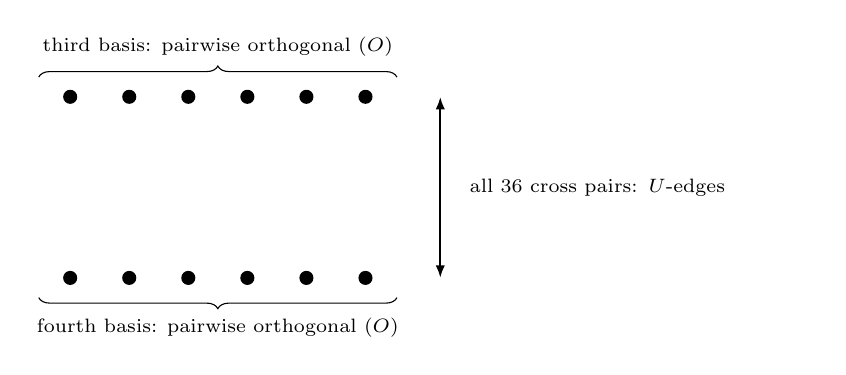
\begin{tikzpicture}[dot/.style={circle,fill,inner sep=1.8pt}]
\foreach \i in {0,...,5} \node[dot] (a\i) at (\i*0.75,1.15) {};
\foreach \i in {0,...,5} \node[dot] (b\i) at (\i*0.75,-1.15) {};
\draw[decorate,decoration={brace,amplitude=4pt}] (-0.4,1.4) -- (4.15,1.4)
  node[midway,above=4pt,font=\scriptsize]{third basis: pairwise orthogonal ($O$)};
\draw[decorate,decoration={brace,amplitude=4pt,mirror}] (-0.4,-1.4) -- (4.15,-1.4)
  node[midway,below=4pt,font=\scriptsize]{fourth basis: pairwise orthogonal ($O$)};
\draw[thick,{Latex[length=1.6mm]}-{Latex[length=1.6mm]}] (4.7,1.15) -- (4.7,-1.15);
\node[font=\scriptsize,anchor=west,text width=4.3cm] at (4.95,0)
  {all $36$ cross pairs: $U$-edges};
\end{tikzpicture}
\end{center}

\begin{center}
\emph{If two further bases exist for some $H$ in the box, the graphs contain two disjoint $6$-cliques
with all $36$ cross edges in $U$.}
\end{center}

\noindent
The proof is the paragraph above: the twelve genuine vectors lie in twelve balls, and every genuine
relation keeps its edge, because an edge is dropped only when the relation is impossible throughout the
balls.

\key{6.\ Why the absence of the pattern is a proof}

The graph search is finite and exact. It fixes the least vertex of the first clique and then keeps, at
every step, only the vertices still adjacent to the partial clique and still available for the second
(the preprint's Lemma 6.8), so it does examine every possible pair of cliques; it answers \emph{no}
only when no such configuration exists, not when it stopped looking. The graph has at most $2048$
vertices, and a step cap of five million guards the search; reaching the cap counts as
\emph{unresolved}, never as a negative answer.

Combine this with the statement in \S5. If the graphs contain no such pair of cliques, then no twelve
vectors with the required pattern exist in the box, so no $H$ in the box extends by two further bases.
Note the direction. The pattern is \emph{necessary} and never sufficient: extra edges only make the
graphs larger, and a larger graph is still a valid refutation tool, because the argument is
``bases $\Rightarrow$ pattern, but no pattern''. What would be fatal is a \emph{missing} edge, and that
cannot happen: an edge is omitted only on the strength of a proof that the relation is impossible
throughout both balls.

This is the sense in which the covering decides the question. We never assume that the two bases exist
and never try to find them. For each box we suppose they exist, derive the pattern, and observe that
the pattern is absent.

\key{7.\ What happens when the pattern survives}

If the graphs do contain the pattern, nothing follows: the box is not refuted and it is not declared
extendible either. It is marked \emph{unresolved} and retested after refinement. A finer bin layer shrinks the vector
balls and tightens the two inequalities of \S5; a subdivided cell of $\U(2)$, or a finer certified phase
ball, shrinks the box and tightens the single-vector and joint tests, so vertices and edges can be
deleted. A possibility the old graphs retained may then be impossible, and the pattern may disappear.
This is the only way a box leaves the unresolved list short of being refuted, and it is why the run has
a prescribed sequence of refinement passes rather than a single test.

The proof is finished when the run has visited every record and none is left unresolved. That is the
content of the preprint's Theorem 7.1: a completed execution implies that no four mutually unbiased
bases exist in $\C^6$.

\key{8.\ The whole argument in one paragraph}

Keep one invariant: \emph{the union of the boxes still on the list contains a representative of every
$H$ that extends by two further bases}. It holds at the start, when one box contains everything. A covering step replaces a
box by finitely many whose union contains it. A refutation deletes a box only when its graphs contain no
pattern, which by \S6 means that no $H$ in the box extends. A refinement replaces a box by smaller boxes
whose union contains it. When the list is empty, the invariant reads: no $H$ extends by two further
bases.

Step 2's contribution is exactly this: it makes each box small. Without it the freedom in $H$ would be
sixteen phases and the errors in \S5 far too large for any edge to be ruled out; with it the freedom is
four angles, the boxes have radius at most $0.03$ cycles, and the tests bite.

\medskip
\noindent\textit{Exercise.} (a) Show that two orthogonal candidate vectors are exactly $\sqrt2$ apart
and two unbiased ones at least $1.08$ apart, so the twelve vectors of \S1 occupy twelve different
balls. (b) Derive the two inequalities of \S5 from $\abs{e(t)-1}\le2\pi\abs t$. (c) Why are extra edges
harmless, while one missing genuine edge would be fatal?

\end{document}
